\chapter{Thermal field theory}

\newcommand{\transampl}{\braket{\phi_B | e^{- i \hat{H} T / \hbar} | \phi_A}}

\section{Summary of quantization of quantum fields}

%TODO: should i have a $t$ as in $\ket{\phi(t)}$ ?)

Consider a quantum field theory with Schrödinger-picture field operators $\hat{\phi}(\vec{x})$ and conjugate momenta $\hat{\pi}(\vec{x})$ and Hamiltonian operator
\begin{equation}
	\hat{H} = \int \dif^3 x \, \ham(\hat{\pi}(\vec{x}), \hat{\phi}(\vec{x})) .
\end{equation}
In analogy with position $x$ and momentum $p$ in classical mechanics, we will refer to $\hat\phi(\vec{x})$ and $\hat\pi(\vec{x})$ as operators in ``position-space'' and ``momentum-space''.
%Whether ``position'' refers to $\vec{x}$ or $\phi(\vec{x})$ will therefore depend on context.

The field operators $\hat{\phi}(\vec{x})$ and $\hat{\pi}(\vec{x})$ have eigenstates $\ket{\phi}$ and $\ket{\pi}$ with corresponding eigenvalues $\phi(\vec{x})$ and $\pi(\vec{x})$ at every point $\vec{x}$, as expressed by the eigenvalue equations
\begin{equation}
	\hat{\phi}(\vec{x}) \ket{\phi} = \phi(\vec{x}) \ket{\phi}
	\qquad \text{and} \qquad
	\hat{\pi}(\vec{x}) \ket{\pi} = \pi(\vec{x}) \ket{\pi} .
\label{eq:tft:field_eigenvalue_equations}
\end{equation}

By assumption, the field and the momentum satisfy the commutation relations
\begin{equation}
	\comm{\hat{\phi}(\vec{x})}{\hat{\pi}(\vec{y})} = i \hbar \delta(\vec{x} - \vec{y})
	\qquad \text{and} \qquad
	\comm{\hat{\phi}(\vec{x})}{\hat{\phi}(\vec{y})} = 
	\comm{\hat{\pi}(\vec{x})}{\hat{\pi}(\vec{y)}} = 
	0
\label{eq:tft:boson_field_commutators}
\end{equation}
for bosons, while for fermions they instead satisfy the anticommutation relations
\begin{equation}
	\acomm{\hat{\phi}(\vec{x})}{\hat{\pi}(\vec{y})} = i \hbar \delta(\vec{x} - \vec{y})
	\qquad \text{and} \qquad
	\acomm{\hat{\phi}(\vec{x})}{\hat{\phi}(\vec{y})} = 
	\acomm{\hat{\pi}(\vec{x})}{\hat{\pi}(\vec{y)}} = 
	0 .
\label{eq:tft:fermion_field_anticommutators}
\end{equation}
% peskin eq. 2.20: in Heisenberg picture, these hold at *equal times*

The position-space eigenstates are orthogonal and complete in the sense
\begin{equation}
	\braket{\phi | \phi'} = \prod_{\vec{x}} \delta(\phi(\vec{x}) - \phi'(\vec{x}))
	\qquad \text{and} \qquad
	\int \dif \phi \ket{\phi} \bra{\phi} = 1 .
	\label{eq:tft:orthogonality_completeness_position}
\end{equation}

\newcommand{\posmom}[2]{\exp \left(  \frac{i}{\hbar} \int \dif^3 x \, #2(\vec{x}) #1(\vec{x}) \right)}
\newcommand{\mompos}[2]{\exp \left( -\frac{i}{\hbar} \int \dif^3 x \, #1(\vec{x}) #2(\vec{x}) \right)}
If we find the inner product $\braket{\phi | \pi}$, we can use it together with the completeness relation \eqref{eq:tft:orthogonality_completeness_position} to express position-space states and momentum-space states in terms of each other through
\begin{equation}
	\ket\pi = \int \dif \phi \ket\phi \braket{\phi | \pi} %= \int \dif \phi \posmom{\phi}{\pi}
	\qquad \text{or} \qquad
	\ket\phi = \int \dif \pi \ket\pi \braket{\pi | \phi} . %= \int \dif \phi \mompos{\pi}{\phi} .
\end{equation}
To do so, let us use the position-space representation $\hat{\pi} = (\hbar / i) \fdv{}/{\phi}$ of the momentum operator.
This gives us a first-order differential equation
\begin{equation}
	\braket{\phi | \hat{\pi} | \pi} = \pi(\vec{x}) \braket{\phi | \pi} = \frac{\hbar}{i} \fdv*{\braket{\phi | \pi}}{\phi}
\end{equation}
for the inner product $\braket{\phi | \pi}$.
Choosing the solution with prefactor $1$, we obtain
\begin{equation}
	\braket{\phi | \pi} = \posmom{\phi}{\pi} .
	\label{eq:tft:inner_product_position_momentum}
\end{equation}

The momentum states are also orthogonal and complete, but with slightly different factors.
Due to our convention \eqref{eq:pre:delta_function} for the delta function, orthogonality takes the form
\begin{equation}
\begin{split}
	\braket{\pi_a | \pi_b} &= \int \dif \phi \braket{\pi_a | \phi} \braket{\phi | \pi_b} \\
	                       &= \int \dif \phi \exp \left( i \int \dif^3 x \, (\pi_b(\vec{x}) - \pi_a(\vec{x})) \phi(\vec{x}) / \hbar \right) \\
						   &= 2 \pi \hbar \, \delta(\pi_a(\vec{x}) - \pi_b(\vec{x})) .
\end{split}
\end{equation}
To find the completeness relation, we postulate it up to a constant $B$.
Consider
%Inserting a complete set of both position and momentum states and using the inner product \eqref{eq:tft:inner_product_position_momentum}, consider
\begin{equation}
\begin{split}
	1 &= \int \frac{\dif \pi(\vec{x})}{B} \ket{\pi} \bra{\pi} \\
	  &= \int \frac{\dif \pi(\vec{x})}{B} \ket{\pi} \int \frac{\dif \pi'(\vec{x})}{B} \int \dif \phi(\vec{x}) \braket{\pi | \phi} \braket{\phi | \pi'} \bra{\pi'} \\
	  &= \int \frac{\dif \pi(\vec{x})}{B} \ket{\pi} \int \frac{\dif \pi'(\vec{x})}{B} \underbrace{\int \dif \phi(\vec{x}) \exp \left( \frac{i}{\hbar} \int \dif^3 x \, \left( \pi'(\vec{x}) - \pi(\vec{x}) \right) \phi(\vec{x}) \right)}_{2 \pi \hbar \, \delta(\pi'(\vec{x}) - \pi(\vec{x}))} \bra{\pi'} \\
	  &= \frac{2 \pi \hbar}{B} \underbrace{\int \frac{\dif \pi(\vec{x})}{B} \ket{\pi} \bra{\pi}}_{1} .
\end{split}
\end{equation}
This would be inconsistent unless $B = 2 \pi \hbar$, so completeness in momentum-space is
\begin{equation}
	\int \frac{\dif \pi(\vec{x})}{2 \pi \hbar} \ket{\pi} \bra{\pi} = 1 .
\end{equation}

\section{Path integral formulation}

When the Hamiltonian $\hat{H}$ is independent of time, a quantum system evolves from an initial state $\ket{\phi_A}$ to the state $e^{-i \hat{H} T / \hbar} \ket{\phi_A}$ during the time $T$ \cite[equation 2.28]{ref:sakurai}.
Later we will study statistical mechanics for a star in thermal equilibrium -- then the Hamiltonian is always independent of time, otherwise the system would not be in equilibrium.
The transition amplitude for going from the state $\ket{\phi_A}$ to a different state $\ket{\phi_B}$ in the time $T$ is therefore
\begin{equation}
	\transampl \qquad (A \rightarrow B) .
	\label{eq:tft:transition_amplitude_intro}
\end{equation}
Let us demonstrate how this transition amplitude can be written as a path integral.
First, split the time interval $T$ into $N$ intervals $\Delta t = T / N$, and decompose the evolution operator $e^{- i \hat{H} T / \hbar}$ into equally many products of $e^{- i \hat{H} \Delta t / \hbar}$ to write
\newcommand\pointarrow[1]{\underset{\underset{\displaystyle #1}{\displaystyle \uparrow}}{}}
\begin{equation}
	\transampl = \braket{\phi_B | e^{- i \hat{H} \Delta t / \hbar} \cdots e^{- i \hat{H} \Delta t / \hbar} \cdots e^{- i \hat{H} \Delta t / \hbar} | \phi_A} .
\end{equation}
%\transampl = \braket{\phi_b | \pointarrow{4} e^{- i H \Delta t} \,\, \cdots \pointarrow{3} e^{- i H \Delta t} \pointarrow{2} \cdots \,\, e^{- i H \Delta t} \pointarrow{1} | \phi_a}
We will take the limit $N \rightarrow \infty$ in the end, so we assume that each interval $\Delta t$ is small.
Now comes the most important trick -- take a deep breath and do the following.
\begin{itemize}
\item Insert $N$ complete sets of \emph{momentum} states $1 = \int \dif \pi_n / (2 \pi \hbar) \ket{\pi_n} \bra{\pi_n}$ to the \emph{left} of every exponential, including the rightmost one, with $n$ increasing from right to left.
\item Insert $N-1$ complete sets of \emph{position} states $1 = \int \dif \phi_n \ket{\phi_n} \bra{\phi_n}$ to the \emph{right} of every exponential, excluding the rightmost one, with $n$ increasing from right to left.
\end{itemize}
Now exhale.
With this trick, the transition amplitude can be written as the product
\begin{equation}
	\transampl = \prod_{n=0}^{N} \int \frac{\dif \phi_n \dif \pi_n}{2 \pi \hbar} 
	             \braket{\phi_{n+1} | \pi_n} \braket{\pi_n | e^{- i \hat{H} \Delta t / \hbar} | \phi_n} ,
\label{eq:tft:transition_amplitude_product}
\end{equation}
where we have defined $\ket{\phi_0} = \ket{\phi_A}$ and $\ket{\phi_{N+1}} = \ket{\phi_B}$.
The inner products $\braket{\phi_{n+1} | \pi_n}$ can simply be replaced by the exponential \eqref{eq:tft:inner_product_position_momentum}, so let us turn our attention to the matrix elements $\braket{\pi_n | e^{- i \hat{H} \Delta t / \hbar} | \phi_n}$.
Since the time step $\Delta t$ is assumed small, we can expand the exponential $e^{- i \hat{H} \Delta t / \hbar} \taylor 1 - i \hat{H} \Delta t / \hbar$ to first order in time.
Under the assumption that the Hamiltonian $\hat{H}$ is a sum of terms with all \emph{position}-space operators $\hat{\phi}$ on the \emph{right} and all \emph{momentum}-space operators $\hat{\pi}$ on the \emph{left}, we can pull it out of the product at the additional benefit of replacing its operators by their eigenvalues.
We then obtain
\begin{equation}
\begin{split}
	\braket{\pi_n | e^{- i \hat{H} \Delta t / \hbar} | \phi_n} &\taylor \braket{\pi_n | (1 - i \hat{H} \Delta t / \hbar) | \phi_n} \\
	                                                   &=       \braket{\pi_n | \phi_n} (1 - i H_n \Delta t / \hbar) \\
	                                                   &\taylor \braket{\pi_n | \phi_n} e^{- i H_n \Delta t / \hbar}, \\
\end{split}
\label{eq:tft:path_integral_hamiltonian_assumption}
\end{equation}
where we no longer have any operators, but only the Hamiltonian eigenvalue at the $n$-th timestep
\begin{equation}
	H_n = \int \dif^3 x \, \ham(\pi_n(\vec{x}), \phi_n(\vec{x})) .
\label{eq:tft:hamiltonian_eigenvalues}
\end{equation}
Note the importance of expanding the exponential to first order in timeonly.
If the Hamiltonian contained \emph{any} mixed sequence of operators such as $H \propto \hat{\pi} \hat{\phi}$, then higher powers like $\hat{H}^2 \propto \hat{\pi} \hat{\phi} \hat{\pi} \hat{\phi}$ in the power series expansion of the time evolution operator would not be in the assumed left-right order.

(TODO: spør Jens Oluf om et alternativt argument her -- kan ikke bare operatorer i $\hat{H}$ kommuteres inntil man får den ønskede rekkefølgen, samtidig som ekstra konstanter medfører en fysisk ubetydelig fase? F.eks. $\hat{H} = \hat{p} \hat{q} = \hat{q} \hat{p} \pm i \hbar$, men de to har forskjellige egenverdier $pq$ og $pq \pm i \hbar$??? Men dette er alltid en fysisk ubetydelig fase?)

\iffalse
(TODO: If the Hamiltonian is \emph{not} in the order we assumed above, we could always bring it into this order by commuting operators using the commutation relation \eqref{eq:tft:boson_field_commutators}.
But such terms would appear only as a constant phase on the right side of \eqref{eq:tft:path_integral_hamiltonian_assumption} that would not depend on the dynamics of the process.
AHence, we can relax this assumption by absorbing this physically irrelevant phase into the transition amplitude. ER DETTE RIKTIG? INGEN LÆREBØKER NEVNER DETTE.)

(TODO: if this argument holds, then it can be applied for any $\hat{H}^n$, and there is no reason to expand to first order in time, either)
\fi

\begin{figure}
\centering
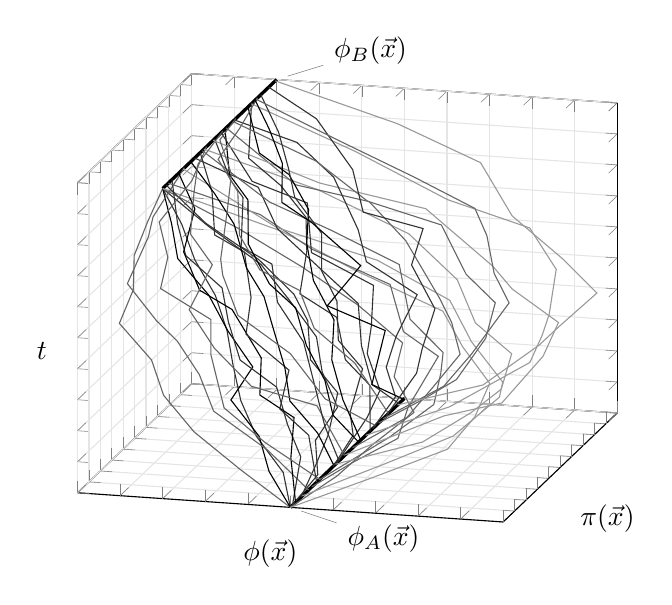
\begin{tikzpicture}
\begin{axis}[
	clip=false,
	view={-75}{20}, 
	%xtick=\empty, ytick=\empty, ztick=\empty, 
	xticklabel=\empty, yticklabel=\empty, zticklabel=\empty,
	xlabel=$\pi(\vec{x})$, ylabel=$\phi(\vec{x})$, zlabel=$t$, zlabel style={rotate=-90},
	%x label style={at={(axis description cs:0.5,0.0)},anchor=north},
	%y label style={at={(axis description cs:0.5,0.0)},anchor=north},
	%z label style={at={(axis description cs:0.5,0.0)},anchor=north},
	xmin=0, xmax=1, ymin=0, ymax=1, zmin=0, zmax=5,
	xtick distance=0.1, ytick distance=0.1, ztick distance=0.5, grid=major, grid style={solid, thin, black!10!white},
	%extra x ticks={0j
	declare function={
		phi1 = 0.5;
		phi2 = 0.8;
		randbetween(\a,\b) = \a + (\b - \a) / 2 * rand;
		%randradius(\x, \rmin, \rmax) = randbetween(\rmin, \rmax) * (\x-0) * (\x-1);
		randfunc(\x,\rmin,\rmax) = randbetween(\rmin,\rmax) * (\x-0)*(\x-1) * 4; % and(x>=0.01, x<=0.99); %(\x-0) * (\x-1);
	},
]
\addplot3 [domain=0:1, samples=2, very thick] ({x}, {phi1}, {0}) node [pos=0.0,pin={-8:$\phi_A(\vec{x})$}] {};
\addplot3 [domain=0:1, samples=2, very thick] ({x}, {phi2}, {5}) node [pos=1.0,pin={+5:$\phi_B(\vec{x})$}] {};
\pgfplotsinvokeforeach{0.0, 0.2, ..., 1.0} {
	\addplot3 [domain=0:1, samples=10, domain y=0:1, samples y=1, black!60!white]  ({max(0, min(1, #1+randbetween(-0.1,0.1))}, {phi1 + (phi2-phi1)*x + randfunc(x,-0.2,-0.3)}, {5*x});
	\addplot3 [domain=0:1, samples=10, domain y=0:1, samples y=1, black!80!white]  ({max(0, min(1, #1+randbetween(-0.1,0.1))}, {phi1 + (phi2-phi1)*x + randfunc(x,-0.0,-0.1)}, {5*x});
	\addplot3 [domain=0:1, samples=10, domain y=0:1, samples y=1, black!100!white] ({max(0, min(1, #1+randbetween(-0.1,0.1))}, {phi1 + (phi2-phi1)*x + randfunc(x,+0.0,+0.1)}, {5*x});
	\addplot3 [domain=0:1, samples=10, domain y=0:1, samples y=1, black!80!white]  ({max(0, min(1, #1+randbetween(-0.1,0.1))}, {phi1 + (phi2-phi1)*x + randfunc(x,+0.2,+0.3)}, {5*x});
	\addplot3 [domain=0:1, samples=10, domain y=0:1, samples y=1, black!60!white]  ({max(0, min(1, #1+randbetween(-0.1,0.1))}, {phi1 + (phi2-phi1)*x + randfunc(x,+0.4,+0.5)}, {5*x});
	\addplot3 [domain=0:1, samples=10, domain y=0:1, samples y=1, black!40!white]  ({max(0, min(1, #1+randbetween(-0.1,0.1))}, {phi1 + (phi2-phi1)*x + randfunc(x,+0.6,+0.7)}, {5*x});
	%\addplot3 [domain=0:1, samples=10, domain y=0:1, samples y=1] ({#1+randfunc(x,0.2,0.3)}, {phi1 + (phi2-phi1)*x + randfunc(x,0.1,0.2)}, {5*x});
}
\end{axis}
\end{tikzpicture}
\caption{\label{fig:phase_space}A quantum system that evolves from the initial field $\phi_A(\vec{x})$ to the final field $\phi_B(\vec{x})$ can take all possible paths through phase space, but some are more likely than others. The conjugate momentum field $\pi(\vec{x})$ does not need to be the same at the start and the end.}
\end{figure}

Substituting \cref{eq:tft:inner_product_position_momentum,eq:tft:path_integral_hamiltonian_assumption,eq:tft:hamiltonian_eigenvalues}, the transition amplitude \eqref{eq:tft:transition_amplitude_product} becomes
\begin{equation}
\begin{split}
	\transampl &=      \left( \prod_{n=1}^N \int \frac{\dif \phi_n \dif \pi_n}{2 \pi \hbar} \right) \\
	           &\times \exp \left( \frac{i \Delta t}{\hbar} \sum_{n=1}^N \int \dif^3 x \left( \pi_n(\vec{x}) \frac{\phi_{n+1}(\vec{x}) - \phi_n(\vec{x})}{\Delta t} - \ham(\pi_n(\vec{x}), \phi_n(\vec{x})) \right)
	\right)
\end{split}
\end{equation}
Finally, we take the continuum limit by sending $N \rightarrow \infty$.
It is then natural to define
$\phi(\vec{x}, t_n) = \phi_n(\vec{x}, t_n)$
and
$\pi(\vec{x}, t_n) = \pi_n(\vec{x}, t_n)$
to be the values of the fields at each timestep $t_n$.
Both become continuous functions of time in the continuum limit.
We also use the finite difference definition of the derivative to turn the fraction in the exponential into a partial derivative $\dot{\phi}(\vec{x},t) = \pdv{\phi(\vec{x},t)}/{t}$.
Similarly, we use the Riemann sum definition of the integral to turn the sum $\sum \Delta t$ into an integral $\int \dif t$.
We also define the \textbf{functional integrals}
\begin{equation}
	\int \pathintdif \phi = \lim_{N \rightarrow \infty} \prod_{n=1}^{N} \int \dif \phi_n
	\qquad \text{and} \qquad
	\int \pathintdif \pi = \lim_{N \rightarrow \infty} \prod_{n=1}^{N} \int \frac{\dif \pi_n}{2 \pi \hbar} .
\end{equation}
%We have swept the diverging factor $(2 \pi \hbar)^N$ under the rug, arguing that it contains no physical information about the dynamics of the process and can be ignored, unlike the other factors.
%TODO: can integrate out momentum with gaussian integral if it appears as $p^2$)
With all of these steps, the transition amplitude takes the form of the \textbf{path integral}
\begin{equation}
\begin{split}
	\transampl &=      \int \pathintdif \pi \int_{\phi(\vec{x}, 0)=\phi_A(\vec{x})}^{\phi(\vec{x},T)=\phi_B(\vec{x})} \pathintdif \phi \\
	           &\times \exp \left( \frac{i}{\hbar} \int_0^T \dif t \int \dif^3 x \left( \pi(\vec{x}, t) \dot{\phi}(\vec{x}, t) - \ham(\pi(\vec{x}, t), \phi(\vec{x}, t)) \right) \right) .
\end{split}
\label{eq:tft:path_integral_hamiltonian}
\end{equation}

(TODO: mention/do Legendre transformation to $\lagr = \pi \dot{\phi} - \ham$?)

\iffalse
Note that the combination of the Hamiltonian and the fields in the exponential is precisely the Legendre transformation that converts between the Hamiltonian density $\ham$ and the Lagrangian density $\lagr$.
Thus, we might as well express the transition amplitude as the \textbf{path integral}
%	\transampl = \int \pathintdif \pi \int_{\phi_A(\vec{x}, 0)}^{\phi_B(\vec{x}, T)} \pathintdif \phi \\
%	             \exp \left( i \int_0^T \dif t \int \dif^3 x \, \left( \lagr(\pi(\vec{x}, t), \phi(\vec{x}, t)) \right) \right) .
\begin{equation}
	\transampl = \int \pathintdif \pi \int_{\phi_A(\vec{x})}^{\phi_B(\vec{x})} \pathintdif \phi \, \exp \big( i S \left[ \pi(\vec{x}, t), \phi(\vec{x}, t) \right] / \hbar \big) ,
\label{eq:tft:path_integral_lagrangian}
\end{equation}
with the action
\begin{equation}
	S \left[ \pi(\vec{x}, t), \phi(\vec{x}, t) \right] = \int_0^T \dif t \int \dif^3 x \, \lagr \left( \pi(\vec{x}, t), \phi(\vec{x}, t) \right) . \qquad \text{TODO: factor $c$?}
\label{eq:tft:action}
\end{equation}
\fi
The path integral expresses the transition amplitude for the process $A \rightarrow B$ as a sum over all possible paths through phase space, each weighted by the value on the unit circle with phase corresponding to the action of the path.
This interpretation is illustrated in \cref{fig:phase_space}.
Note that the position-space integral $\int \pathintdif \phi$ is constrained to start and end in the initial and final states, but the momentum integral $\int \pathintdif \pi$ has no such constraint at the endpoints.

(TODO: the only ``correct'' way is to do this AGAIN for fermions!)

\section{Partition function}

We will now see that there is an elegant mathematical analogy between the path integral for the transition amplitude and the partition function of statistical mechanics.
In a quantum system, the partition function in the grand canonical ensemble is
\begin{equation}
	Z = \trace \left( e^{-\beta (\hat{H} - \mu_i \hat{N}_i)} \right) = e^{-\beta \Omega} ,
\end{equation}
where $\beta = 1 / k_B T$, $\mu_i$ are chemical potentials, $\hat{N}_i$ are number operators, $\Omega = -k_B T \log{Z}$ is the grand potential and the trace can be evaluated in any basis.
If we can find the partition function, we can obtain thermodynamic information such as \cite[chapter 5]{ref:jensoluf}
\begin{align}
	%\text{the entropy}                     \quad \thermalavg{S}   &= -\pdv{\Omega}{T} \\
	           & \text{the average number of particles} & \thermalavg{N_i} & = k_B T \pdv{\log{Z}}{\mu_i},                    & \\
	           & \text{the average energy}              & \thermalavg{E}   & = \mu_i \thermalavg{N_i} - \pdv{\log{Z}}{\beta}  & \\ % \Omega + T S + \mu_i \thermalavg{N_i} \\
	\text{and} & \text{the average pressure}            & \thermalavg{P}   & = \frac{k_B T}{V} \log{Z}.                       &    % -\pdv{\Omega}{V}
\end{align}
This is exactly what we eventually want to insert into the TOV equation \eqref{eq:tov}.
We could, of course, evaluate the partition function in the basis of fields $\ket{\phi_0}$, where
\begin{equation}
	Z = \int \dif \phi_0 \braket{\phi_0 | e^{-\beta (\hat{H} - \mu_i \hat{N}_i)} | \phi_0} .
\end{equation}
This is precisely an integral over transition amplitudes \eqref{eq:tft:path_integral_hamiltonian}, but now with 
\begin{itemize}
\item equal start and end states $\ket{\phi_A} = \ket{\phi_B} = \ket{\phi_0}$, 
\item the Hamiltonian $\hat{H} - \mu_i \hat{N}_i$ and 
\item a purely imaginary time variable $t = -i \tau$ with $\tau$ running from $0$ to $\beta \hbar$.
\end{itemize}
The change from a real to imaginary time variable can be accomplished by a Wick rotation that does not change the value of the integral (TODO: true?).
Thus, we can express the partition function as path integrals \eqref{eq:tft:path_integral_hamiltonian} with these substitutions!
This yields
\begin{equation}
	Z = \int \pathintdif \pi \oint \pathintdif \phi \, \exp \left( \frac{1}{\hbar} \int_0^{\beta \hbar} \dif \tau \int \dif^3 x \left( i \pi(\vec{x}, \tau) \dot{\phi}(\vec{x}, \tau) - \ham(\pi(\vec{x}, \tau), \phi(\vec{x}, \tau)) \right) \right)
\label{eq:tft:partition_function}
\end{equation}
where we have absorbed $\int \dif \phi_0$ into the path integral $\int \pathintdif \phi$ and write $\oint$ to indicate that we integrate over all fields $\phi(x, \tau) = \phi(x, \tau + \beta \hbar) \, e^{i \theta}$ that are \emph{periodic} in imaginary time, due to the equal start and end states $\phi_A(\vec{x}) = \phi_B(\vec{x})$ in \cref{eq:tft:path_integral_hamiltonian}.
We take a general approach by allowing periodicity up to an arbitrary phase factor $e^{i \theta}$ -- we will see shortly that $e^{i \theta} = +1$ for bosonic fields and $e^{i \theta} = -1$ for fermionic fields.
(TODO: this is bullshit, the integral explicitly says the field should be ``normal-periodic'' -- the only way to show this properly is by doing the path integral again for fermions)
Thus, thermal field theory -- statistical mechanics for quantum fields at finite temperature -- is essentially equivalent to ordinary quantum field theory with temperature-dependent time and periodic fields, and the partition function is obtained by integrating along closed paths in phase space!

\section{Matsubara frequencies}

The periodicity $\psi(x, 0) = \psi(x, \beta \hbar) \, e^{i \theta}$ in time ensures that we can expand the field as a Fourier series
\begin{equation}
	\psi(x, \tau) = \sum_n \psi_n(x) e^{i \omega_n \tau}
\end{equation}

The \textbf{Matsubara frequencies} $\omega_n$ are restricted by the bosonic or fermionic nature of the field.
To see this, consider the (TODO: thermal?) Green's function
\begin{equation}
	G_\pm (\vec{x}, \vec{y}, \tau_1, \tau_2) = Z^{-1} \, \trace{\left\{ e^{-\beta (\hat{H} - \mu \hat{N})} \right\}} = \ldots
\end{equation}
To see this, write commutators generally by
\begin{equation}
	\comm{A}{B}_\pm = \ldots
\end{equation}
The Matsubara frequencies are thus
\begin{equation}
	\omega_n = \begin{cases}
			       2 \pi n / \beta \hbar    & \text{(bosons)} \\
				   (2n+1) \pi / \beta \hbar & \text{(fermions)} \\
	           \end{cases}
\end{equation}

The field is not periodic in \emph{space}, but we can still take the Fourier \emph{transform}
\begin{equation}
	\psi_n(x) = \int \frac{\dif^3 p}{(2 \pi \hbar / L)^3} \, \psi_n(\vec{p}) e^{i \vec{p} \cdot \vec{x} / \hbar}
\end{equation}
Thus, we can expand
\begin{equation}
	\psi(x, \tau) = \sum_n \sum_\vec{p} \psi_n(\vec{p}) e^{i (\vec{p} \cdot \vec{x} / \hbar + \omega_n \tau)}
	\qquad \text{where} \qquad
	\sum_\vec{p} = V \int \frac{\dif^3 p}{(2 \pi \hbar)^3} .
\end{equation}

(TODO: general Matsubara frequencies for bosons/fermions!)

\section{Bosons}

(TODO: do Bose-Einstein with complex scalar field instead of real scalar field for more ``symmetry'' to the fermionic case?)

For a real scalar field, the Lagrangian is 
(TODO: does this define the unit of $\phi$ is such that unit of $\lagr$ is $\text{energy} / \text{volume}$?, i.e. $[\phi] = \sqrt{E/M}$?)
(TODO: did something wrong with time derivative -- with or without $c$?)
\begin{equation}
	\lagr = \frac{1}{2 c^2} (\partial_\mu \phi) (\partial^\mu \phi) - \frac12 \frac{m^2 c^2}{\hbar^2} \phi^2
	      = \frac{1}{2 c^2} \dot{\phi}^2 - \frac12 (\nabla \phi)^2 - \frac12 \frac{m^2 c^2}{\hbar^2} \phi^2 .
\end{equation}
The conjugate momentum is defined as
\begin{equation}
	\pi = \pdv{\lagr}{\dot{\phi}} = \frac{1}{c^2} \dot{\phi} .
\end{equation}
The Hamiltonian density is therefore
\begin{equation}
	\ham = \pi \dot{\phi} - \lagr = \frac12 c^2 \pi^2 + \frac12 (\nabla \phi)^2 + \frac12 \frac{m^2 c^2}{\hbar^2} \phi^2 .
\label{eq:tft:boson_hamiltonian}
\end{equation}
We can now calculate the partition function \eqref{eq:tft:partition_function}.
Substituting the Hamiltonian density \eqref{eq:tft:boson_hamiltonian} gives
\begin{equation}
	Z = \int \pathintdif \pi \oint \pathintdif \phi \exp \left\{ \frac{1}{\hbar} \int_0^{\beta \hbar} \dif \tau \int \dif^3 x \left[ i \pi \dot{\phi} - \frac12 c^2 \pi^2 - \frac12 (\nabla \phi)^2 - \frac12 \frac{m^2 c^2}{\hbar^2} \phi^2 \right] \right\} .
\end{equation}
We can integrate away the momenta with a Gaussian integral by completing the square for $i \pi \dot{\phi} - \frac12 c^2 \pi^2 = -\frac12 c^2 (\pi - i \phi / c^2)^2 - \frac12 \frac{1}{c^2} \dot{\phi}^2$ and then shifting $\pi \rightarrow \pi - i \phi / c^2 = \pi'$.
More precisely,
\begin{equation}
\begin{split}
	Z & =       \int \pathintdif \pi  \oint \pathintdif \phi \exp \left\{ \frac{1}{\hbar} \int_0^{\beta \hbar} \dif \tau \int \dif^3 x \left[ -\frac{c^2}{2} \left( \pi - \frac{i \phi}{c^2}\right )^2 - \frac{1}{2 c^2} \dot{\phi}^2 - \frac12 (\nabla \phi)^2 - \frac12 \frac{m^2 c^2}{\hbar^2} \phi^2 \right] \right\} \\
	  & =       \int \pathintdif \pi' \oint \pathintdif \phi \exp \left\{ \frac{1}{\hbar} \int_0^{\beta \hbar} \dif \tau \int \dif^3 x \left[ -\frac{c^2}{2} \pi'^2                                    - \frac{1}{2 c^2} \dot{\phi}^2 - \frac12 (\nabla \phi)^2 - \frac12 \frac{m^2 c^2}{\hbar^2} \phi^2 \right] \right\} \\
	  & \propto                       \oint \pathintdif \phi \exp \left\{ \frac{1}{\hbar} \underbrace{\int_0^{\beta \hbar} \dif \tau \int \dif^3 x \left[                                              - \frac{1}{2 c^2} \dot{\phi}^2 - \frac12 (\nabla \phi)^2 - \frac12 \frac{m^2 c^2}{\hbar^2} \phi^2 \right] }_{S} \right\} .
\end{split}
\label{eq:tft:boson_partition_function_momentum_out}
\end{equation}
In the last line we used the Gaussian integral $\int_{-\infty}^{+\infty} \dif x \, e^{-x^2} = \sqrt{\pi}$ with a suitable rescaling of $x$ (where $\pi \approx 3.1415$, of course -- not the conjugate momentum).
We do not bother keeping track of this constant or any other constants in front of the partition function, as the physical quantities only contain derivatives of the logarithm of $Z$ (TODO: ref. but this statement is not true for the pressure!).
Thus it only remains to tackle the position-space integral over $\phi$.

The action in the exponent of the partition function \eqref{eq:tft:boson_partition_function_momentum_out} has no variation at the boundaries, so we can integrate it by parts and forget about boundary terms.
We can thus write it in the form
\begin{equation}
\begin{split}
	S & = \int_0^{\beta \hbar} \dif \tau \int \dif^3 x \left[ - \frac{1}{2c^2} \pdv{\phi}{\tau}^2 - \frac12 (\nabla \phi)^2 - \frac12 \frac{m^2 c^2}{\hbar^2} \phi^2 \right] \\
	  & = \int_0^{\beta \hbar} \dif \tau \int \dif^3 x \, \phi \left[ \frac{1}{2c^2} \pdv[2]{}{\tau} + \frac12 \nabla^2 - \frac12 \frac{m^2 c^2}{\hbar^2} \right] \phi .
\end{split}
\end{equation}
To proceed, let us use periodicity of the field to expand it in a Fourier series
\begin{equation}
\begin{split}
	\phi(\vec{x}, \tau) & = \hbar c \, \sqrt{\frac{\beta}{V}} \sum_{n=-\infty}^{+\infty} \sum_{\vec{p}}       \phi_n(\vec{p})  e^{+i (\vec{p} \cdot \vec{x} / \hbar + \omega_n \tau)} \\
	                    & = \hbar c \, \sqrt{\frac{\beta}{V}} \sum_{n=-\infty}^{+\infty} \sum_{\vec{p}} \conj{\phi_n(\vec{p})} e^{-i (\vec{p} \cdot \vec{x} / \hbar + \omega_n \tau)} .
\end{split}
\end{equation}
The prefactor $\hbar c \sqrt{\beta/V}$ is chosen to have the same dimension as the position-space field $\phi(\vec{x}, \tau)$, so the Fourier amplitudes $\phi_n(\vec{p})$ are dimensionless.
Without it, the Gaussian integral that we will end up computing in \cref{eq:tft:boson_gaussian_integral} would make the partition function $Z$ dimensionful, which would formally make it meaningless to take its logarithm.

(TODO: make a ``checkpoint'' here by noting that the partition function can always be written as a functional determinant, so always restart here instead of restarting the game every time)

Perhaps deceptively, we made it look like we represented the positional part of $\psi(\vec{x}, \tau)$ by a Fourier series too, suggesting it is periodic.
But it is \emph{not} -- it is only the imaginary \emph{time} that we showed was periodic.
What we \emph{actually} do is to represent it by a Fourier transform, but we \emph{write} it as a discrete Fourier sum.
We really mean to take the continumm limit
\begin{equation}
	\sum_\vec{p} = \int \frac{\dif^3 p}{\Delta p} = V \int \frac{\dif^3 p}{(2 \pi \hbar)^3} ,
\end{equation}
where the volume $\Delta p = (2 \pi \hbar)^3 / V$ of the cells $\rightarrow 0$.
The summation signs will make everything more ``compatible'' with the products that will show up shortly.

(TODO: better argument for prefactor? best argument I have: $Z$ in the end should be dimensionless by its definition, so we must add prefactors here to make it so, thus the prefactors in Gale's book!)

In Fourier space, then, the action becomes
(TODO: is underbrace with $\delta$ and $V$ correct?)
\begin{equation}
\begin{split}
	S & = -\frac12 \frac{\hbar^2 c^2 \beta}{V}
	      \sum_{n,m} \sum_{\vec{p},\vec{q}} 
	  	  \phi_m(\vec{q}) 
	  	  \left[ \frac{\omega_n^2}{c^2} + \vec{k}^2 + \frac{m^2 c^2}{\hbar^2} \right] 
		  \phi_{n}(\vec{p})
		  \underbrace{\int \dif^3 x \, e^{i (\vec{p} - \vec{q}) \cdot \vec{x} / \hbar}}_{\delta(\vec{p}-\vec{q}) V}
	      \underbrace{\int_0^{\beta \hbar} \dif \tau \, e^{i (\omega_n - \omega_m) \tau}}_{\delta_{m,n} \beta \hbar}
		  \\
	  & = -\frac12 \hbar^3 \beta^2
	      \sum_n \sum_\vec{p}
	  	  \left[ \omega_n^2 + \omega(\vec{p})^2 \right] 
		  \abs{\phi_{n}(\vec{p})}^2 ,
\end{split}
\end{equation}
where we defined $\omega(\vec{p})$ by $\hbar \omega(\vec{p}) = \sqrt{\vec{p}^2 c^2 + m^2 c^4}$.
As we insert this action into the path integral \eqref{eq:tft:boson_partition_function_momentum_out}, it factors into the Gaussian integrals
\begin{equation}
\begin{split}
	Z & \propto 
	\prod_{n} \prod_{\vec{p}}
	\left\{
		\int \dif \phi_n(\vec{p}) \,
		\exp \left[
			-\frac12 \hbar^2 \beta^2 \left(
				\omega_n^2 + \omega(\vec{p})^2
			\right)
			\abs{\phi_n(\vec{p})}^2
		\right]
	\right\} \\
	  & \propto
	\prod_{n} \prod_{\vec{p}} \left[ 
		\hbar^2 \beta^2 \left( 
			\omega_n^2 + \omega(\vec{p})^2
		\right)
	\right]^{-1/2}
\end{split}
\label{eq:tft:boson_gaussian_integral}
\end{equation}
The logarithm is
\begin{equation}
	\log Z = -\frac12 \sum_n \sum_\vec{p} 
	         \log \left[ \beta^2 \hbar^2 \left( \omega_n^2 + \omega(\vec{p})^2 \right) \right]
\end{equation}
This expression may look pretty enough on its own, but we can push further.
First, use the definite integral
\begin{equation}
	\int_{a^2}^{b^2} \frac{\dif x^2}{x^2 + c^2} = \log(b^2 + c^2) - \log(a^2 + c^2)
\label{eq:tft:integral_trick}
\end{equation}
with $c = \hbar \beta \omega_n$, $b = \hbar \beta \omega$ and any value of $a$ to convert the logarithm into an integral.
Next, recall that $\omega_n = 2 \pi n / \beta \hbar = n \omega_1$ and use
\begin{equation}
	\sum_{n=-\infty}^{+\infty} \frac{1}{(2 \pi n)^2 + x^2} = \frac{1}{2 x} \left( 1 + \frac{2}{e^x - 1} \right)
	%\sum_{n=-\infty}^{+\infty} \frac{1}{n^2 + x^2} = \frac{\pi}{x} \left( 1 + \frac{2}{e^{2 \pi x} - 1} \right)
\end{equation}
to rewrite the integrand.
(TODO: drop second log term)
Then
\begin{equation}
\begin{split}
	\log Z & = -\frac12 \sum_\vec{p} \sum_n \int^{\beta^2 \hbar^2 \omega^2} \frac{\dif x^2}{x^2 + (2 \pi n)^2} \\
	       & = -\frac12 \sum_\vec{p}        \int^{\beta^2 \hbar^2 \omega^2} \frac{\dif x^2}{2 x} \left( 1 + \frac{2}{e^x - 1} \right) \\
	       & = -\frac12 \sum_\vec{p}        \int^{\beta   \hbar   \omega  }       \dif x         \left( 1 + \frac{2}{e^x - 1} \right) \\
	       & =          \sum_\vec{p}        \left[  \frac12 \beta \hbar \omega - \log(e^{\beta \hbar \omega} - 1) \right] \\
	       & =          \sum_\vec{p}        \left[ -\frac12 \beta \hbar \omega - \log(1 - e^{-\beta \hbar \omega}) \right] \\
\end{split}
\end{equation}
Finally, we take the continuous limit in which $\sum_\vec{p} \rightarrow V \int \dif^3 p / (2 \pi \hbar)^3$, so
\begin{equation}
	\log Z = V \int \frac{\dif^3 p}{(2 \pi \hbar)^3} \left[ -\frac12 \beta \hbar \omega - \log(e^{-\beta \hbar \omega}) \right] .
	\qquad \text{TODO: $V$ how?}
\end{equation}

(TODO: use functional determinant instead?)

(TODO: $\omega = 2 \pi n / \beta \hbar$ ?)

\section{Fermions}

Dirac lagrangian
\begin{equation}
	\lagr = \bar\psi (i \hbar c \slashed\partial - m c^2) \psi
\end{equation}
where $\psi$ is the basic field and $\bar\psi = \psi^\dagger \gamma^0$.
(TODO: gamma matrices)

Conjugate momentum
\begin{equation}
	\pi = \pdv{\lagr}{\dot{\psi}} = i \hbar \psi^\dagger
\end{equation}

Hamiltonian density
\begin{equation}
	\ham = \pi \dot\psi - \lagr = \bar\psi ( -i \hbar c \, \vec{\gamma} \cdot \vec{\nabla} + m c^2 ) \psi
\end{equation}

Fourier series
\begin{equation}
	\psi_\alpha(\vec{x}, \tau) = \frac{1}{\sqrt{V}} \sum_n \sum_\vec{p} e^{i (\vec{p} \cdot \vec{x} / \hbar + \omega_n \tau)} \psi_{\alpha, n}(\vec{p})
\end{equation}
with $\omega_n = (2n+1) \pi / \beta \hbar$.

Partition function
(TODO: conserved current)
\begin{equation}
	Z = \int \pathintdif [i \hbar \psi^\dagger] \int \pathintdif 
	    \exp \left\{ \frac{1}{\hbar} \int_0^{\beta \hbar} \dif \tau \int \dif^3 x \, \bar\psi \left[ -\hbar \gamma^0 \pdv{}{\tau} + i \hbar c \vec{\gamma} \cdot \vec{\nabla} - mc^2 + \mu \gamma^0 \right] \psi \right\}
\end{equation}

Action
\begin{equation}
\begin{split}
	S & = \frac{1}{V} \sum_{m,n} \sum_{\vec{p},\vec{q}}         \psi_m(\vec{q})^\dagger \gamma^0 \left[ -\hbar \gamma^0 i \omega_n + i \hbar c \vec{\gamma} \cdot i \vec{k} - m c^2 + \mu \gamma^0 \right] \psi_n(\vec{p}) \int_0^{\beta \hbar} \dif \tau e^{i(\omega_n-\omega_m)\tau} \int \dif^3 x e^{i(\vec{p}-\vec{q})\cdot\vec{x}/\hbar} \\
	  & = \beta       \sum_{n}   \sum_{\vec{p}}         i \hbar \psi_m(\vec{q})^\dagger          \left[ -\hbar \omega_n + i c \gamma^0 \vec{\gamma} \cdot \vec{p} + i m c^2 \gamma^0 - i \mu \right] \psi_n(\vec{p}) \\
\end{split}
\end{equation}
so
\begin{equation}
\begin{split}
	Z & = \prod_n \prod_\vec{p} \int \pathintdif [i \hbar \psi_n(\vec{p})^\dagger] \int \pathintdif \psi_n(\vec{p})
	      \exp \left\{ \frac{\beta}{\hbar} i \hbar \psi_n(\vec{q})^\dagger \left[ -\hbar \omega_n + i c \gamma^0 \vec{\gamma} \cdot \vec{p} + i mc^2 \gamma^0 - i \mu \right] \psi_n(\vec{p}) \right\} \\
	  & = \prod_n \prod_\vec{p} \int \dif [i \psi_n(\vec{p})^\dagger] \int \dif \psi_n(\vec{p})
	      \exp \left\{ i \psi_n(\vec{q})^\dagger \left[ \beta( -\hbar \omega_n + i c \gamma^0 \vec{\gamma} \cdot \vec{p} + i mc^2 \gamma^0 - i \mu ) \right] \psi_n(\vec{p}) \right\} \\
	  & = \prod_n \prod_\vec{p} \tdet D_n(\vec{p})
\end{split}
\end{equation}
(TODO: $\dif$ or $\pathintdif$ ??)

Using $\int \dif \bar\eta \int \dif \eta e^{\eta^\dagger D \eta} = \det{D}$, we get
\begin{equation}
	\log Z = \trace{\log{D}}
\end{equation}

Determinant
\begin{equation}
\begin{split}
	\tdet D  & = \tdet \left\{ -\beta \hbar \omega_n - i \beta \mu + i \beta m c^2 \gamma^0 + i \beta c \gamma^0 \vec{\gamma} \cdot \vec{p} \right\} \\
	         & = \tdet \begin{pmatrix} 
	                 -\beta \hbar \omega_n - i \beta \mu + i \beta m c^2           & i \beta c \vec{\sigma} \cdot \vec{p}                \\ 
	                 i \beta c \vec{\sigma} \cdot \vec{p}                          & -\beta \hbar \omega_n - i \beta \mu - i \beta m c^2 \\ 
	             \end{pmatrix} \\
	         & = \tdet \left\{ (-\beta \hbar \omega_n - i \beta \mu + i \beta mc^2) (-\beta \hbar \omega_n - i \beta \mu - i \beta m c^2) + \beta^2 c^2 (\vec{\sigma} \cdot \vec{p})^2 \right\} \\
	         & = \tdet \left\{ (-\beta \hbar \omega_n - i \beta \mu)^2 + (\beta m c^2)^2 + \beta^2 c^2 \underbrace{(\vec{\sigma} \cdot \vec{p})^2}_{\vec{p}^2} \right\} \\
	         & = \tdet \left\{ \beta^2 \left[ (\hbar \omega_n + i \mu)^2 + \hbar^2 \omega^2 \right] \right\} \\
	         & = \beta^4 \left[ (\hbar \omega_n + i \mu)^2 + \hbar^2 \omega^2 \right]^2
\end{split}
\end{equation}
(TODO: to 4th or 2nd power when taking determinant of diagonal matrix?)

Now
\begin{equation}
\begin{split}
	\log Z & = \sum_n \sum_\vec{p} \tdet D_n(\vec{p}) \\
	       & = \sum_n \sum_\vec{p} \log \beta^4 \left[ (\hbar \omega_n + i \mu)^2 + \hbar^2 \omega^2 \right]^2 \\
	       & = \sum_n \sum_\vec{p} \log \beta^4 \left[ (\hbar \omega_n + i \mu)^2 + \hbar^2 \omega^2 \right] \left[ (-\hbar \omega_n + i \mu)^2 + \hbar^2 \omega^2 \right] \\
	       & = \sum_n \sum_\vec{p} \log \beta^4 \left[ \hbar^2 \omega_n^2 + 2 i \hbar \omega_n \mu - \mu^2 + \hbar^2 \omega^2 \right] \left[ \hbar^2 \omega_n^2 - 2 i \hbar \omega_n \mu - \mu^2 + \hbar^2 \omega^2 \right] \\
	       & = \sum_n \sum_\vec{p} \log \beta^4 \left[ \hbar \omega_n + i (\hbar \omega + \mu) \right] 
		                                        \left[ \hbar \omega_n + i (\hbar \omega - \mu) \right]
		                                        \left[ \hbar \omega_n - i (\hbar \omega + \mu) \right]
		                                        \left[ \hbar \omega_n - i (\hbar \omega - \mu) \right] \\
	       & = \sum_n \sum_\vec{p} \log \beta^4 \left[ \hbar^2 \omega_n^2 + (\hbar \omega - \mu)^2 \right] 
		                                        \left[ \hbar^2 \omega_n^2 + (\hbar \omega + \mu)^2 \right] \\
	       & = \sum_n \sum_\vec{p} \left\{ \log \beta^2 \left[ \hbar^2 \omega_n^2 + (\hbar \omega - \mu)^2 \right] +
		                                   \log \beta^2 \left[ \hbar^2 \omega_n^2 + (\hbar \omega + \mu)^2 \right] \right\}
\end{split}
\end{equation}
(got rid of the weird $i \mu$ in the beginning)

(can do this ``trickery'' since we sum over all frequencies $\sum_n \omega_n = 0$ and $\sum_n F(\omega_n) = \sum_n F(-\omega_n)$)

Now again use \eqref{eq:tft:integral_trick} with $c = \hbar \beta \omega_n$, $b = \beta ( \hbar \omega \pm \mu )$ and any value of $a$.
(TODO: generalize Matsubara frequency sum)
Next, use
\begin{equation}
	\sum_{n=-\infty}^{+\infty} \frac{1}{(2n+1)^2\pi^2 + x^2} = \frac{1}{2x} \left( 1 - \frac{2}{e^x+1} \right)
\end{equation}
Then
\begin{equation}
\begin{split}
	\log Z_\pm & = \sum_n \sum_\vec{p} \int^{\beta^2 (\hbar \omega \pm \mu)^2} \frac{\dif x^2}{x^2 + (2n+1)^2\pi^2} \\
	           & =        \sum_\vec{p} \int^{\beta^2 (\hbar \omega \pm \mu)^2} \frac{\dif x^2}{2 x} \left( 1 - \frac{2}{e^x +1} \right) \\
	           & =        \sum_\vec{p} \int^{\beta   (\hbar \omega \pm \mu)  }       \dif x         \left( 1 - \frac{2}{e^x +1} \right) \\
	           & =        \sum_\vec{p} \left[ -(\hbar \omega \pm \mu) + 2 \log \left( e^{\beta (\hbar \omega \pm \mu)} + 1 \right) \right]    \\
	           & =        \sum_\vec{p} \left[ +(\hbar \omega \pm \mu) + 2 \log \left( 1 + e^{-(\beta (\hbar \omega \pm \mu))} \right) \right] \\
\end{split}
\end{equation}
and
\begin{equation}
	\log Z %= \log Z_+ + \log Z_-
	       = 2 V \int \frac{\dif^3 p}{(2 \pi \hbar)^3} \left[ \hbar \omega + \log \left( 1 + e^{-\beta (\hbar \omega + \mu)} \right) + \log \left( 1 + e^{-\beta (\hbar \omega - \mu)} \right) \right]
\end{equation}
